\chapter{Génération, simulation et reconstruction des événements}

\section{Reconstruction des événements}

\subsection{L'algorithme \emph{Particle-Flow} (PF)}

CMS utilise un algorithme spécialisé pour reconstruire les objets physiques : l'algorithme du \emph{particle-flow} \citep{pf,cms_pf_2,cms_pf_jets,cms_pf_leptons}. En utilisant l'information de tous les sous-détecteurs pour reconstruire l'événement, cet algorithme permet d'améliorer significativement la résolution des particules reconstruire, et s'avère être un moyen efficace de contrebalancer la résolution moyenne de HCAL : on peut en effet utiliser l'excellente performance du trajectographe pour aider à la reconstruction des hadrons chargés.


Le \emph{particle-flow} permet de reconstruire les 5 types de particules stables détectées par CMS : les électrons, les muons, les photons, et les hadrons neutres et chargés. Toutes les autres particules ont en effet des temps de vie trop court, et se désintègrent en un ensemble de particules détectables avant d'atteindre les sous-détecteurs. Ces particules sont ensuite utilisés comme des briques élémentaires pour reconstruire des objets plus complexe, comme les jets. Étant ensuite utilisées par les analyses de physiques, il est primordiale que le \emph{particle-flow} possède une efficacité de reconstruction la plus haute possible, tout en ayant un taux de fausse identification le plus faible possible. Ces contraintes ont conduit a l'élaboration d'algorithmes dédiés de trajectographie et de calorimétrie, détaillée ci-dessous.

\subsubsection{Trajectographie itérative} \label{sec:tracks_reconstruction}

L'impulsion des hadrons chargés est mesurée avec une résolution bien meilleure par le trajectographe que par les calorimètres. Comme près de \sfrac{2}{3} de l'énergie d'un jet est dû à la présence de hadrons chargés, le trajectographe joue un rôle majeur dans la performance du \emph{particle-flow}.

Afin de reconstruire les trajectoires des particules avec une grande efficacité, tout en conservant un taux de faux minimale, une procédure itérative \citep{cms_tracks} est employée. La reconstruction commence en utilisant seulement les \emph{hits} des deux première couches du détecteur à pixels, ainsi que la position du point d'interaction. C'est ce qu'on appelle la graine de l'algorithme. On cherche ensuite à compléter la trajectoire en utilisant les \emph{hits} des autres couches du trajectographe. Les contraintes lors de cette première étape sont vraiment forte, ce qui conduit à une efficacité de reconstruction moyenne, mais à un très faible taux de faux.

Avant l'étape suivante, les \emph{hits} associés de façon certaine à une trajectoire sont enlevés de la liste des \emph{hits} disponibles, et on réitère ensuite la même procédure en relâchant un peu les contraintes, ce qui permet d'améliorer l'efficacité de reconstruction, tout en gardant un taux de faux très faible grâce à la réduction de la combinatoire. Après la troisième itération, on obtient une efficacité de reconstruction de \SI{99.5}{\%} pour les muons isolés et de plus de \SI{90}{\%} pour les hadrons chargés. Pour les quatrième et cinquième itérations la contrainte sur le point d'interaction est relâchée, ce qui permet de reconstruire les trajectoires des hadrons chargés secondaires produit après le point d'interaction.

Grâce à cet algorithme de trajectographie itératif, la trajectoire d'une particule chargée ne laissant que 3 \emph{hits}, avec un $p_T$ de seulement \SI{150}{\MeV} et un vertex de production éloigné de plus de \SI{50}{\cm} de l'axe du faisceau est reconstruite avec un taux de faux de l'ordre du pourcent. On peut voir figure \ref{fig:iterative_tracking_eff} l'efficacité de reconstruction des trajectoires grâce à l'utilisation de l'algorithme de trajectographie itératif.

\begin{figure} \centering
  \subcaptionbox{\label{fig:tracking_eff_mu}}[0.45\textwidth]{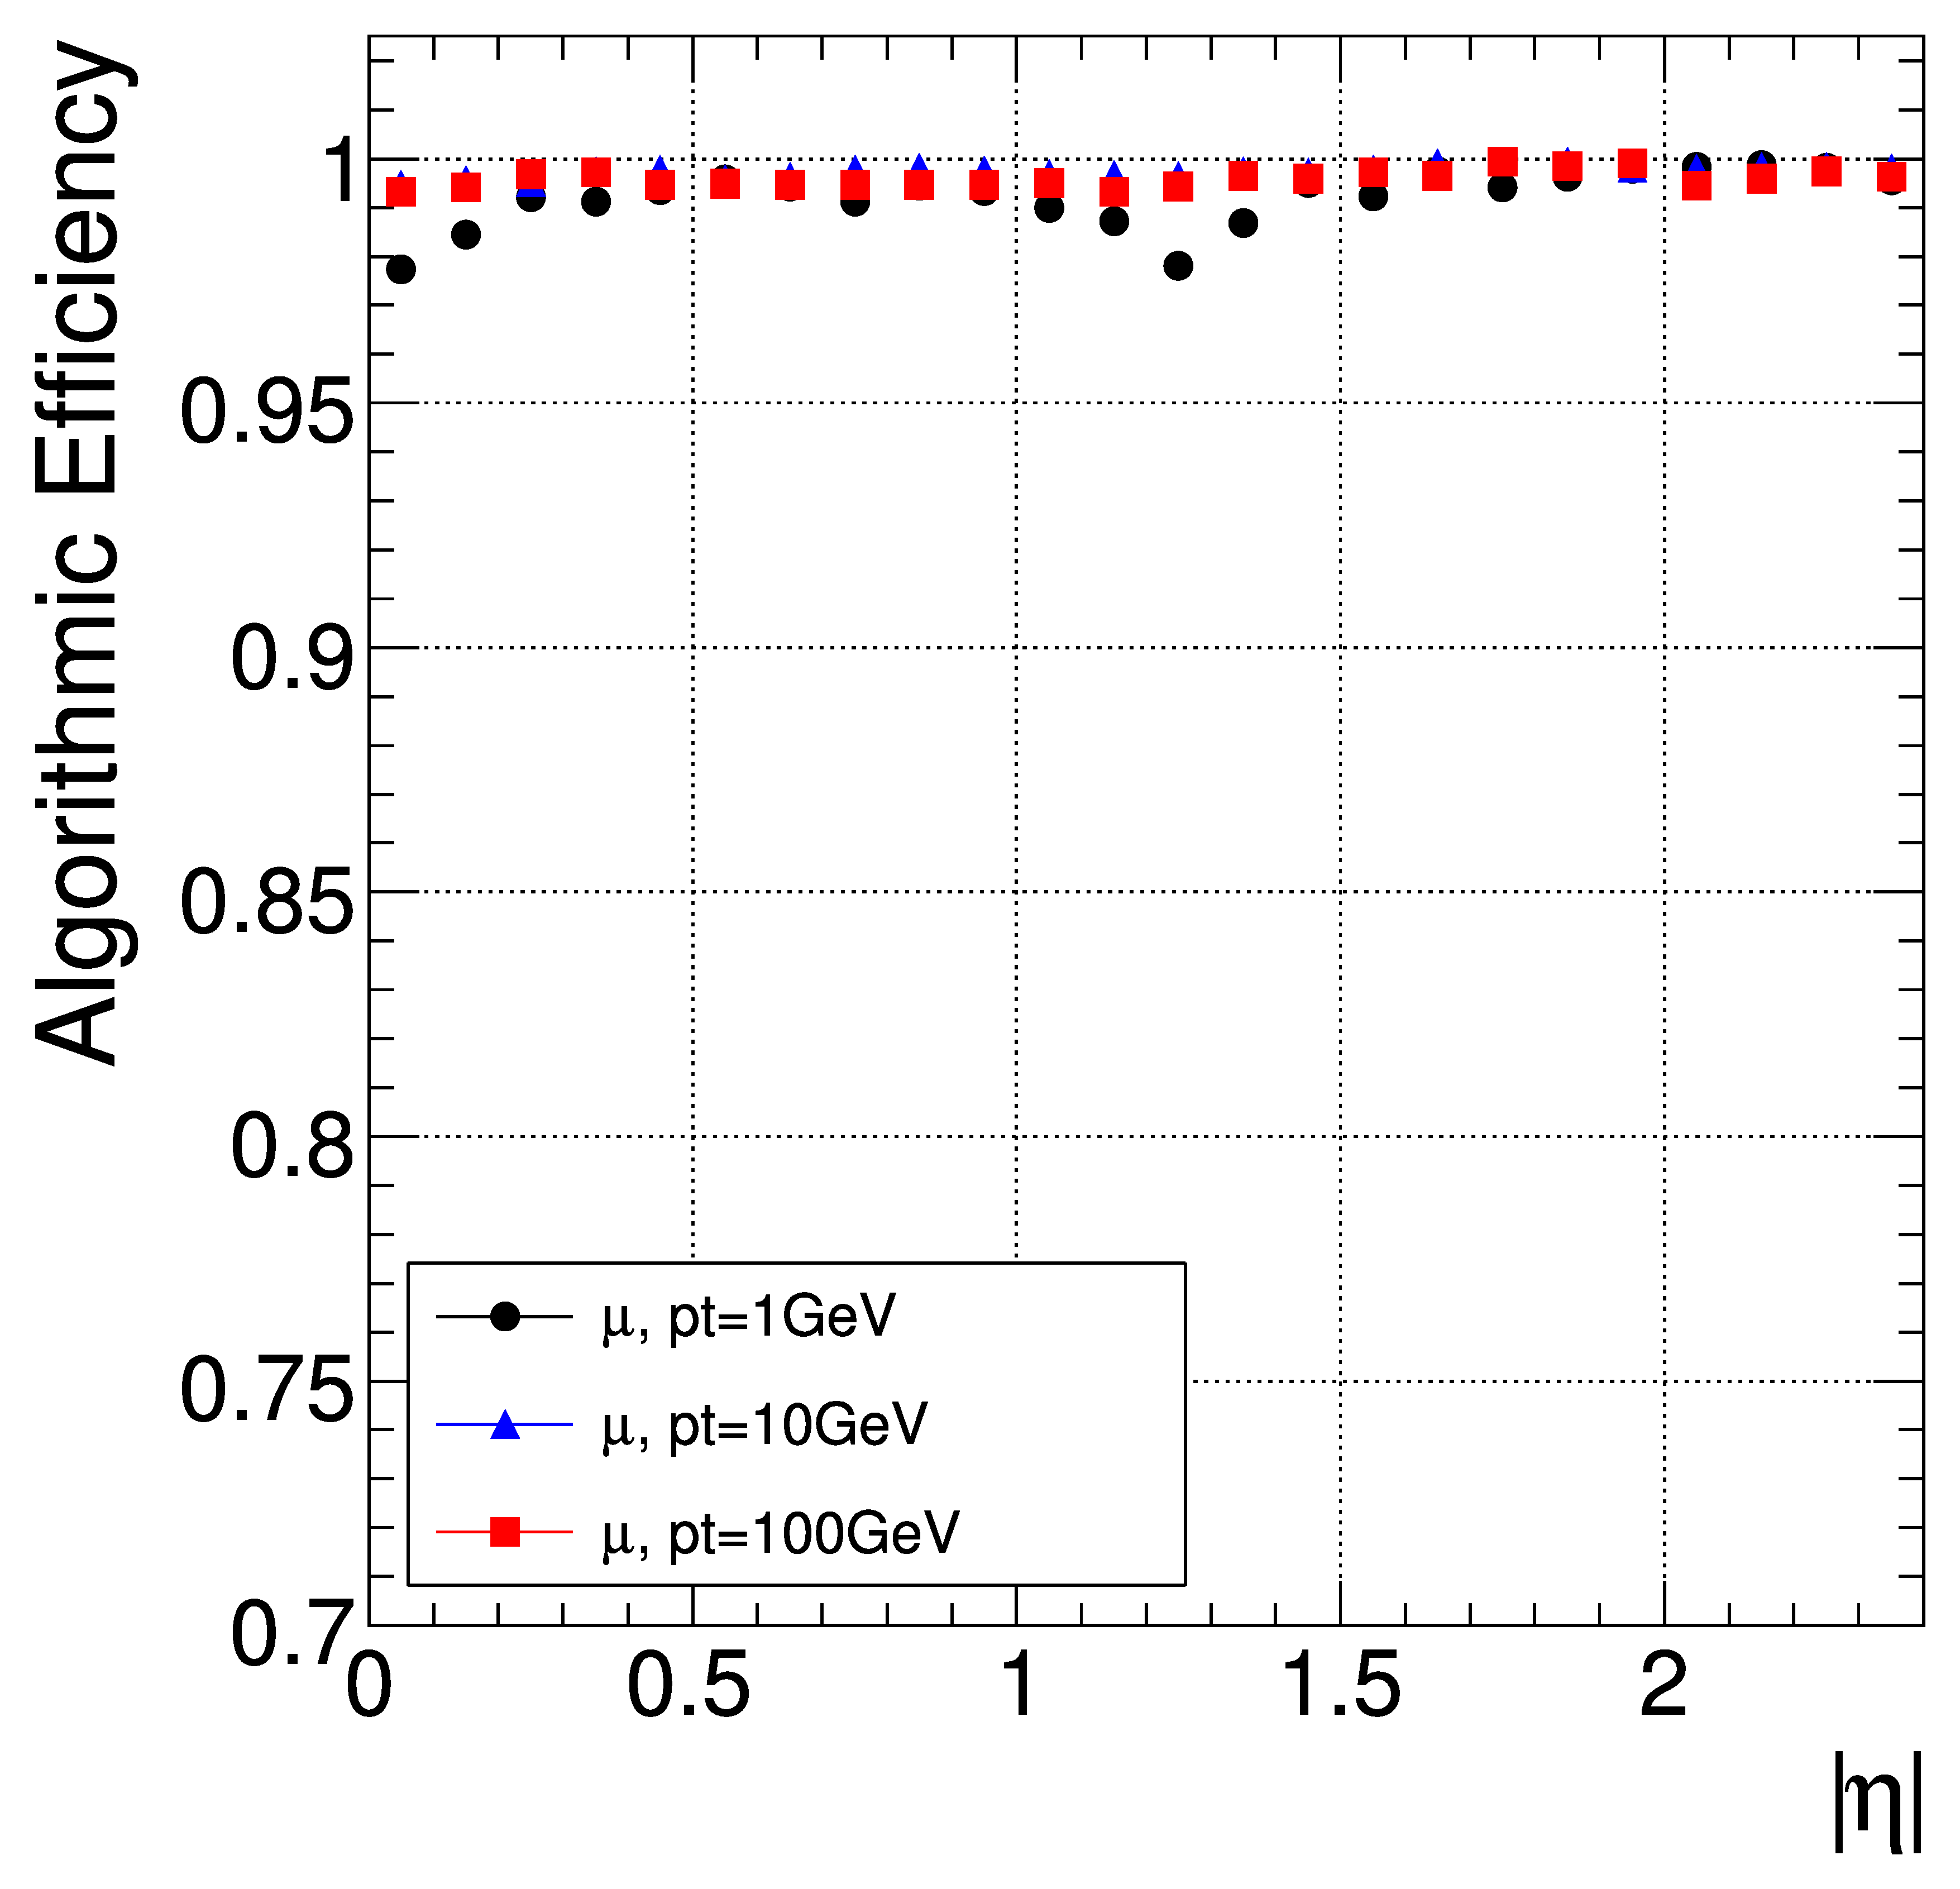
\includegraphics[width=0.45\textwidth]{chapitre3/figs/iterative_tracking_mu.pdf}}\hfill
  \subcaptionbox{\label{fig:tracking_eff_pi}}[0.45\textwidth]{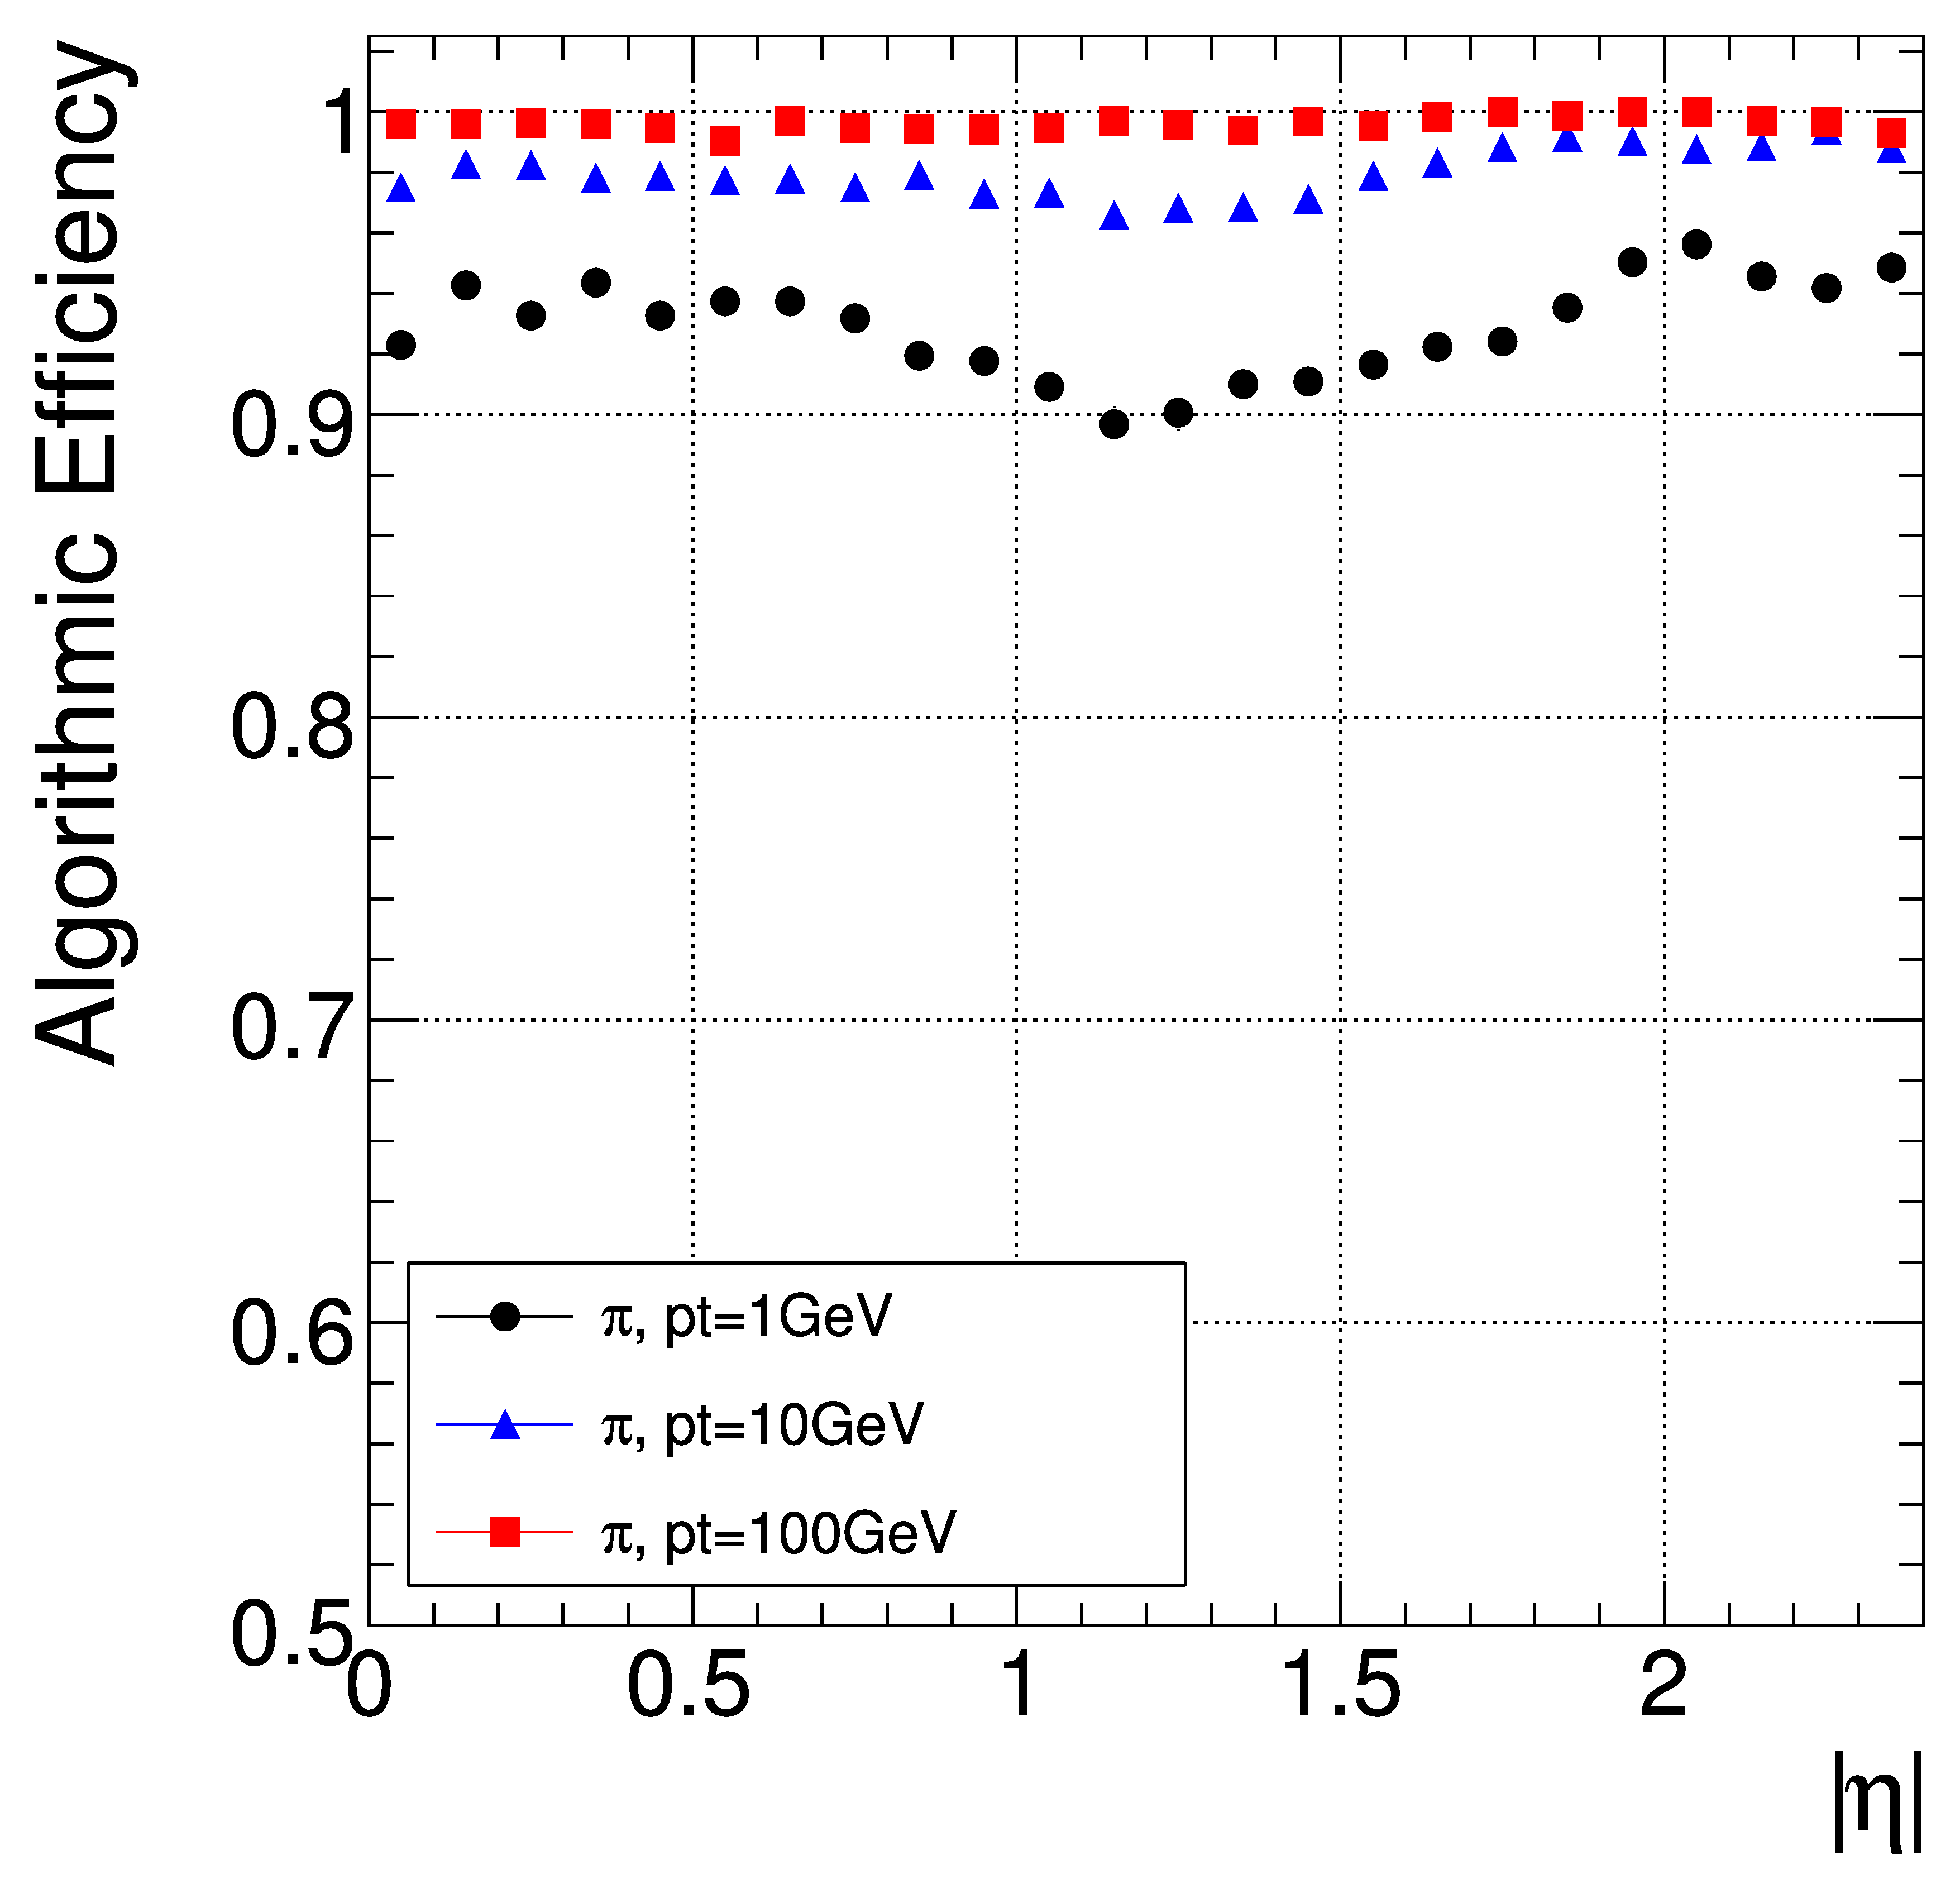
\includegraphics[width=0.45\textwidth]{chapitre3/figs/iterative_tracking_pi.pdf}}
  \caption{Efficacité de reconstruction des trajectoires pour des muons (\subref{fig:tracking_eff_mu}) et pour des pions (\subref{fig:tracking_eff_pi})}
  \label{fig:iterative_tracking_eff}
\end{figure}

\subsubsection{Agglomération calorimétrique}

Un algorithme d'agglomération calorimétrique cherche à atteindre 4 buts : 
\begin{enumerate}
  \item Mesurer l'énergie et la direction des particules neutres (photon, hadrons neutres).
  \item Séparer les dépôts d'énergie des particules neutres de ceux des particules chargées.
  \item Reconstruire les électrons et le rayonnement Bremsstrahlung associé.
  \item Aider à la mesure de l'énergie des hadrons chargés pour lesquels la trajectoire n'a pas été bien reconstruit (hadrons de bas \pt).
\end{enumerate}

L'algorithme spécifique développé pour le \emph{particle-flow} permet d'atteindre une très haute efficacité de reconstruction, tout en gardant un grand pouvoir de séparation des dépôts d'énergie. L'agglomération est effectuée de façon séparée dans chaque sous-calorimètre (tonneau du ECAL, tonneau du HCAL, bouchons du ECAL et HCAL, \ldots), et ce en trois phases.

\medskip

\begin{figure}
  \subcaptionbox{\label{fig:calo_topo}}[0.45\textwidth]{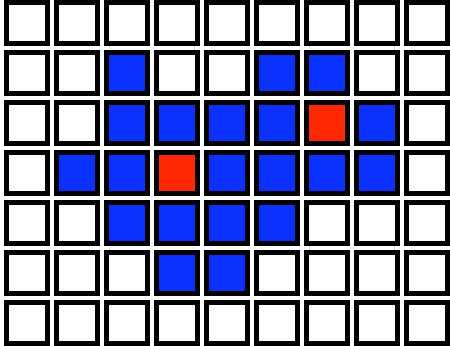
\includegraphics[width=0.45\textwidth]{chapitre3/figs/calo_topoclus_seeds.pdf}}\hfill
  \subcaptionbox{\label{fig:calo_depth}}[0.45\textwidth]{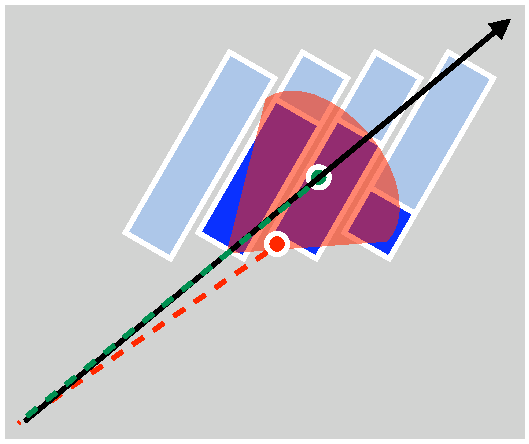
\includegraphics[width=0.45\textwidth]{chapitre3/figs/calo_depthcor.pdf}}
  \caption{Agglomérat topologique contenant deux graines (\subref{fig:calo_topo}) et détermination de la profondeur du dépôt d'énergie (\subref{fig:calo_depth})}
\end{figure}

Premièrement, on identifie les graines de l'algorithme comme les cellules calorimétrique où l'énergie dépasse un certain seuil, fixé arbitrairement mais supérieur au niveau de bruit du détecteur. Les cellules en contact avec une graine (4 ou 8 suivant la configuration) ne peuvent pas devenir des graines à leur tour. On construit ensuite des "agglomérats topologiques", en partant des graines et en agrégeant les cellules avec au moins un côté en commun avec la graine et avec une énergie au dessus d'un seuil, fixé comme deux fois la déviation standard du bruit électronique dans le ECAL (\SI{80}{\MeV} dans le tonneau, \tilde \SI{300}{\MeV} dans les bouchons) et à \SI{800}{\MeV} dans le HCAL. Il peut y avoir plusieurs graines dans un même agglomérat topologique. Dans ce cas, le partage de l'énergie entre chaque graine est effectuée selon la distance entre la cellule et la graine, en considérant que les gerbes électromagnétiques déposent leur énergie selon un profil gaussien, dont la largeur ne dépend pas de l'énergie.

\medskip

La position de l'agrégat est déterminée à partir de la graine et des 4 ou 8 cellules voisines, à l'aide de la formule
\begin{align*}
  X &= \frac{ \sum_i{w_i X_i} }{ \sum_i{w_i} }\text{, avec } w_i = \ln{\frac{E_i}{E_{th}}}
\end{align*}
avec $X = x, y$ ou $z$, $X_i$ la position de la cellule $i$, $E_i$ l'énergie de la cellule $i$, et $E_{th}$ le seuil d'énergie. Dans le cas où l'agrégat ne compte qu'une seule graine, toutes les cellules de l'agrégat sont utilisées pour calculer la position. Afin de ne pas introduire de biais en $\eta$ lors de la détermination de la position, on estime la profondeur du maximum de la gerbe électronique par la formule
\begin{align*}
  p &= a\left( b + \ln{E} \right)
\end{align*}
où $a$ et $b$ sont des constantes qui dépendent de $\eta$, et $E$ l'énergie totale de l'agrégat. On peut voir figure \ref{fig:calo_depth} l'effet de cette procédure sur la détermination de la position angulaire de l'agrégat.

\subsubsection{L'algorithme de liaison} \label{sec:pf_links}

Il reste maintenant à lier ensemble les traces et les agrégats reconstruit puisqu'une particule peut déposer de l'énergie dans les divers sous-détecteurs, tout en éliminant toute possibilité de double comptage de l'énergie. L'algorithme produit donc des "blocs" d'éléments qui vont ensuite servir pour reconstruire les particules. Grâce à l'excellente granularité de CMS, chaque bloc compte en moyenne 2-3 éléments, ce qui permet aux algorithmes de reconstructions des particules de rester extrêmement performant, et ce même quand les événements deviennent très complexes.

\paragraph{Les liens traces – agrégat calorimétrique}

Les traces reconstruites dans le trajectographe sont extrapolées :
\begin{itemize}
  \item Dans le calorimètre électromagnétique, jusqu'à une profondeur correspondant au maximum attendu d'une gerbe électromagnétique \fxnote{Essayer de trouver une distance ? Code ?}
  \item Dans le calorimètre hadronique, jusqu'à une profondeur d'une interaction nucléaire ($\lambda_0$, voir \cref{sec:hcal}), longueur caractéristique d'une gerbe hadronique.
\end{itemize}

On relie la trace à un agrégat si la position extrapolée de la trace passe dans la zone délimitée par l'agrégat. Cette zone peut être augmentée d'une unité (un cristal pour le ECAL, ou une tour pour le HCAL) dans chaque direction, afin de tenir compte de possibles trous entre les modules calorimétriques, de l'incertitude sur la profondeur du maximum de la gerbe, et enfin des multiples diffusions des particules de très bas \pt. On peut voir figure \ref{fig:pf_links} la connexion entre deux traces et des agrégats calorimétriques pour un événement enregistré en décembre 2009 par CMS. On défini la distance du lien par la distance $\Delta R = \sqrt{\eta^2 + \phi^2}$ dans le plan ($\eta$, $\phi$).

\begin{figure}
  \subcaptionbox{ECAL\label{fig:pf_links_ecal}}[0.45\textwidth]{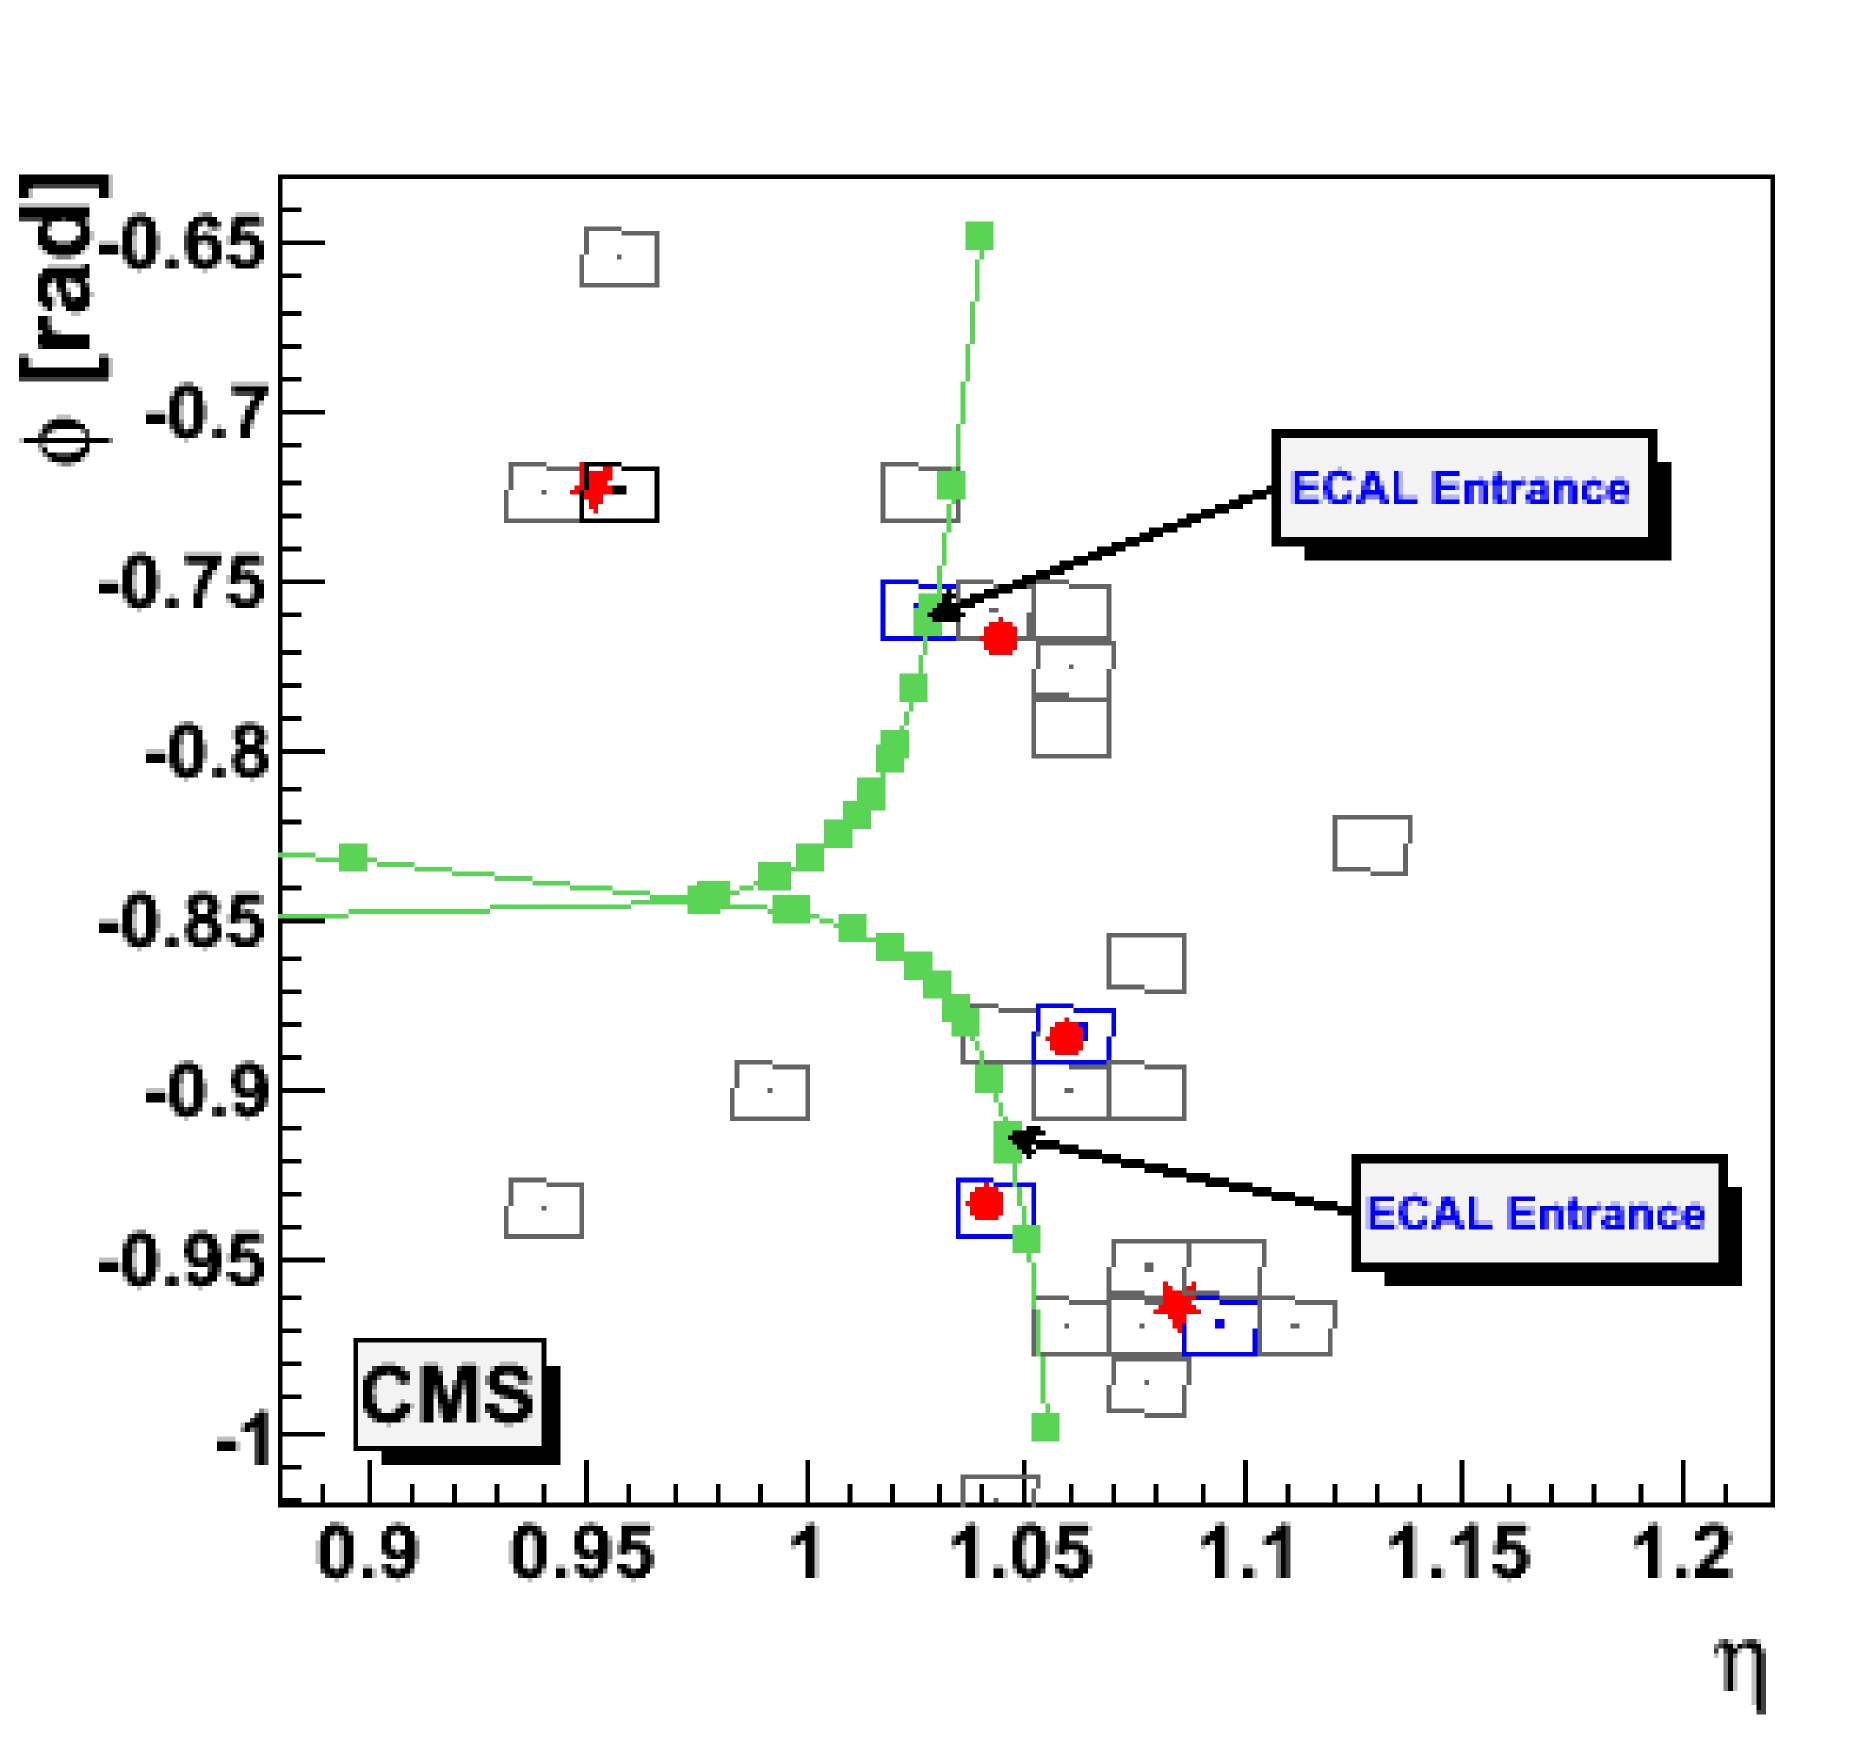
\includegraphics[width=0.45\textwidth]{chapitre3/figs/pf_links_ecal.png}}\hfill
  \subcaptionbox{HCAL\label{fig:pf_links_hcal}}[0.45\textwidth]{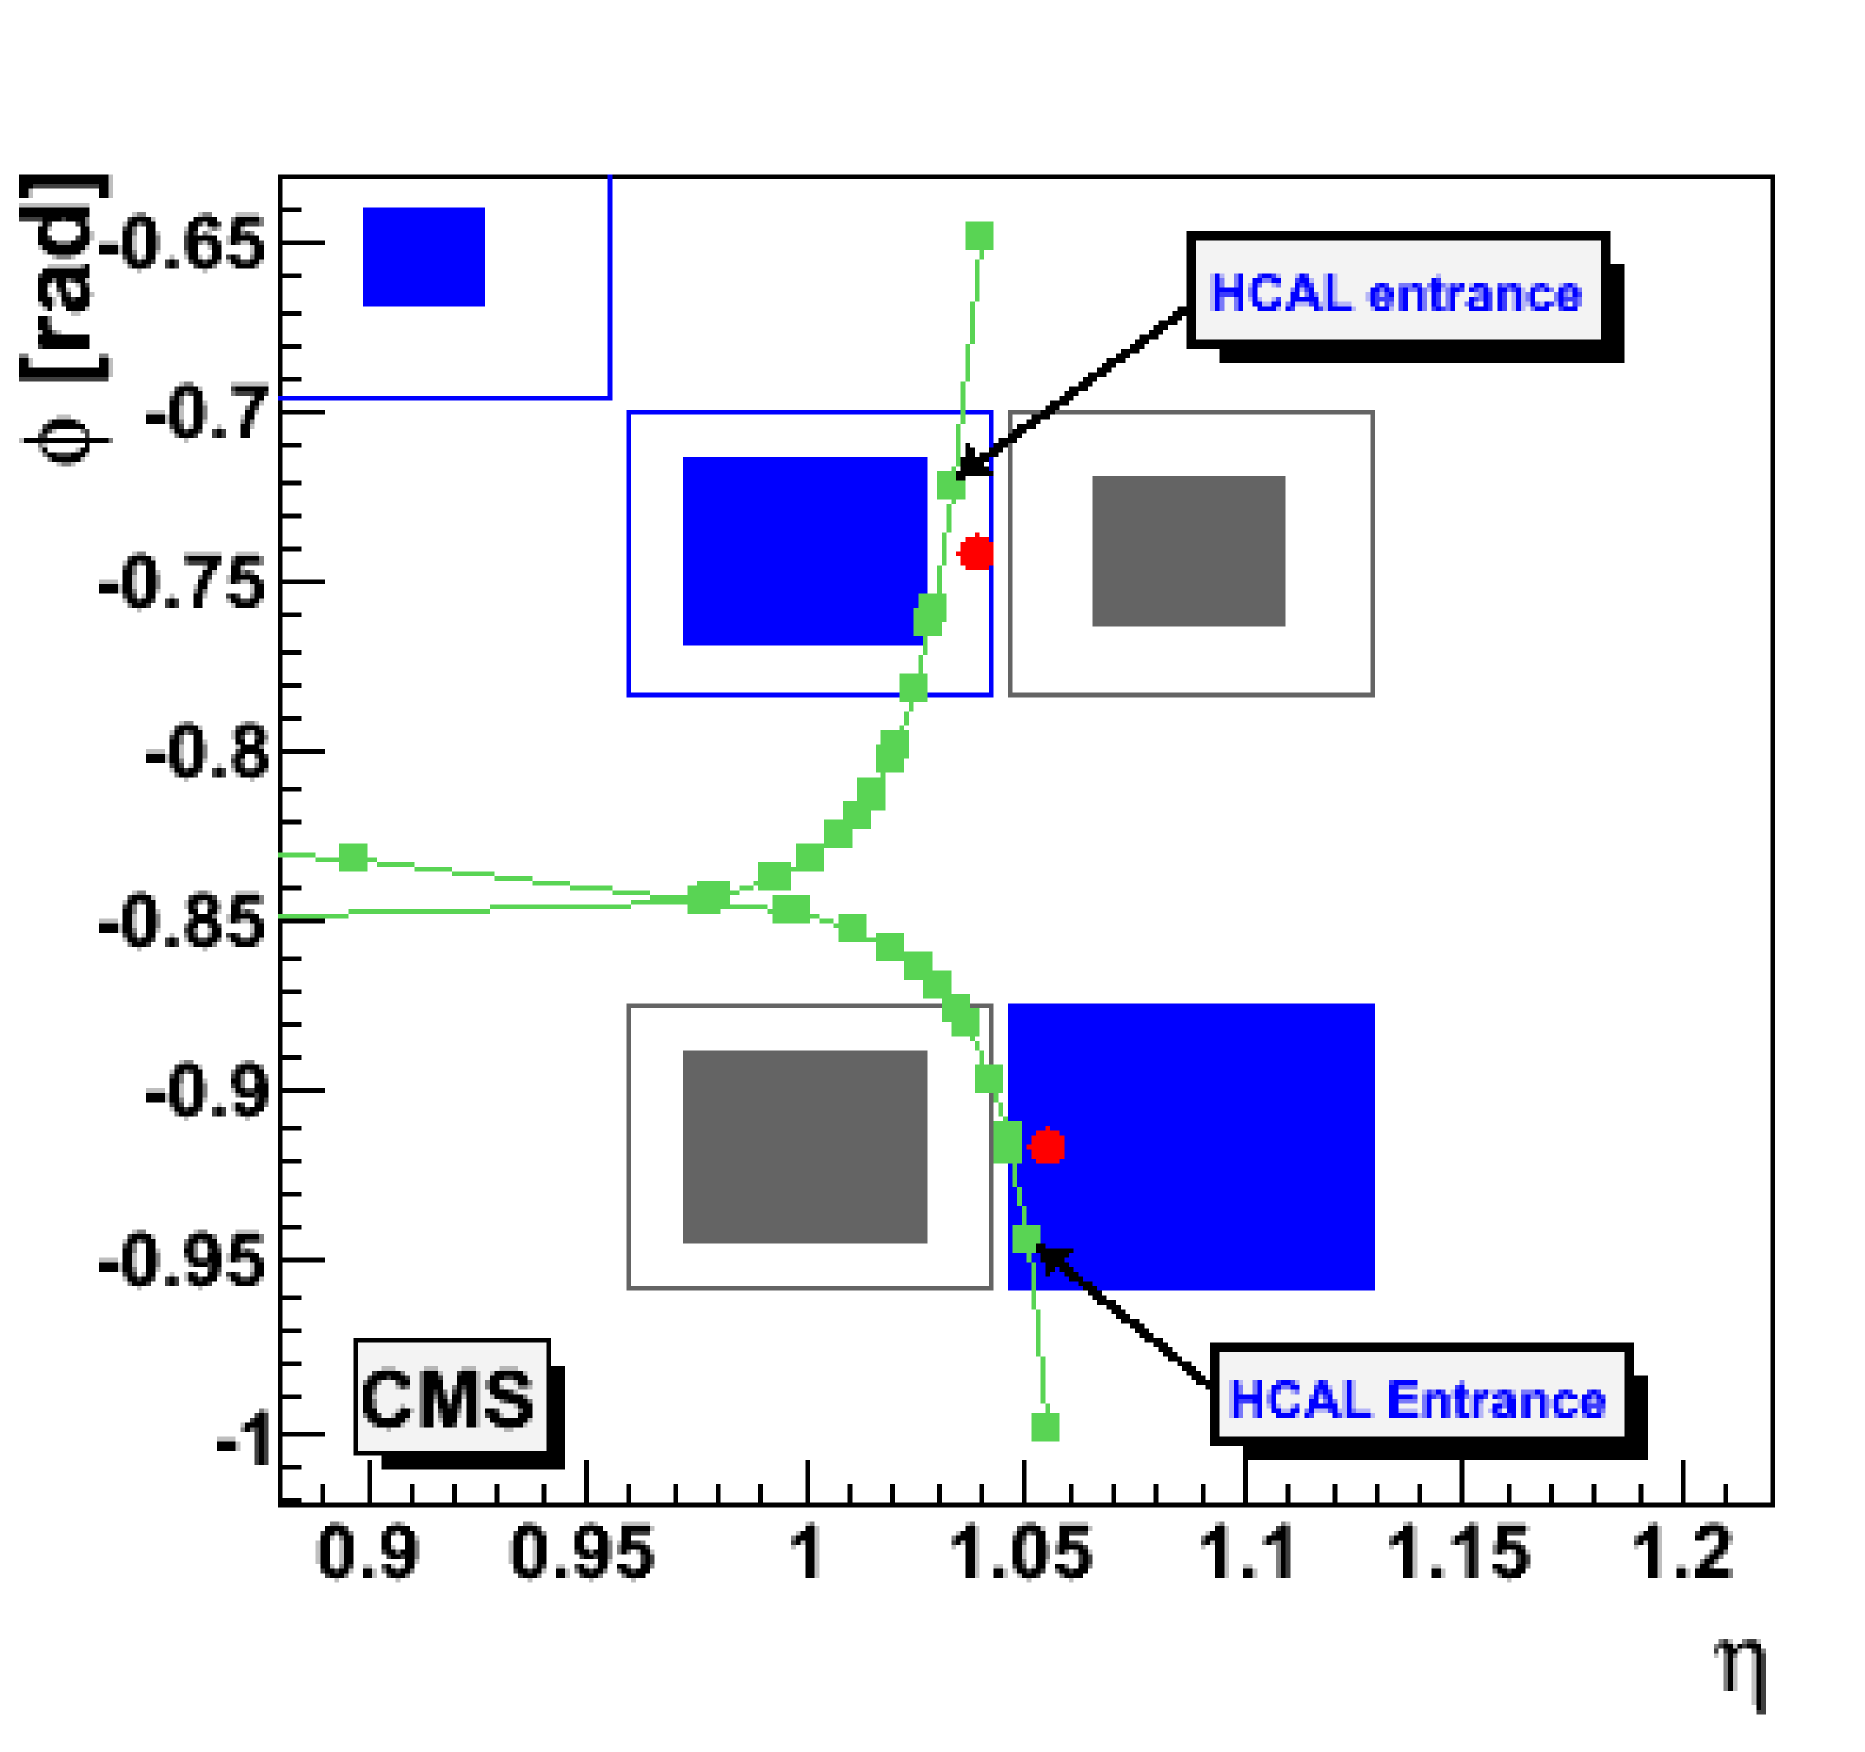
\includegraphics[width=0.45\textwidth]{chapitre3/figs/pf_links_hcal.png}}
  \caption{Connexion entre les traces et les agrégats calorimétrique. Les traces (les lignes vertes avec marqueurs carrés) sont liés avec un ou deux agrégats dans le ECAL (\subref{fig:pf_links_ecal}) et un agrégat dans le HCAL (\subref{fig:pf_links_hcal}). Chaque carré gris représente une cellule calorimétrique. Les ronds rouges représente les agrégats liés à une trace, alors que les étoiles rouges sont les agrégats non liés.}
  \label{fig:pf_links}
\end{figure}

\fxnote{Correction !!!}
In an attempt to collect the energy of all Bremsstrahlung photons emitted by electrons, tangents
to the tracks are extrapolated to the ECAL from the intersection points between the track and
each of the tracker layers. A cluster is linked to the track as a potential Bremsstrahlung photon
if the extrapolated tangent position is within the boundaries of the cluster, as defined above.

\paragraph{Les liens ECAL – HCAL}

De façon similaire, un lien entre les deux calorimètres est créé lorsque la position de l'agrégat formé dans le calorimètre électromagnétique est contenu dans la zone limitée par l'agrégat formé dans le calorimètre hadronique. L'enveloppe des agrégats peut ici aussi être agrandie d'une unité de chaque côté. La distance du lien est ici aussi donné par $\Delta R$ dans le plan ($\eta$, $\phi$).

\paragraph{Les liens trajectographe – détecteur à muons} \label{sec:pf_link_mu}

Le spectromètre à muons reconstruit aussi des traces. Un lien est fait (qu'on appelle muon global) avec les traces du trajectopraphe lorsque l'ajustement entre les deux traces donne un $\chi^2$ acceptable. Si une trace dans le détecteur à muons peut être associée à plusieurs traces dans le trajectographe, le lien est fait entre les deux traces qui donnent le plus petit $\chi^2$. Pour ce type de lien, la distance du lien est donné par le $\chi^2$.

\subsection{L'identification des particules}

Après application de l'algorithme de liaison (voir \cref{sec:pf_links}), on dispose d'une liste de blocs, composés chacun d'environ 2-3 éléments (traces ou agrégats calorimétriques). Il reste maintenant à identifier chaque bloc en tant que particule. Cette identification conduira à la création d'une liste de particule, donnant une description globale de l'événement.

\subsubsection{Reconstruction des muons}

Les premières particules a être reconstruite sont les muons \citep{cms_muons_reco}, avant même le début de la reconstruction de l'événement grâce au \emph{particle-flow}. Les muons laissant des traces à la fois dans le trajectographe et dans le spectromètre à muons, deux types de reconstructions sont utilisées :

\begin{description}
    \item[Reconstruction des muons globaux] Pour chaque trace dans le spectromètre à muons, on cherche par extrapolation une trace correspondante dans le trajectographe, afin de déterminer une trace globale grâce à une interpolation des deux trajectoires. Cette technique est similaire à celle utilisée dans l'algorithme de lien trajectoire -- détecteur à muons présenté \cref{sec:pf_link_mu}. A haute impulsion transverse ($\pt \gtrsim \SI{200}{\GeV}$), cette méthode permet d'améliorer la résolution de l'impulsion comparé à l'utilisation de la trace du trajectographe uniquement.
    \item[Reconstruction des \emph{tracker} muons] On ne considère ici que les traces présentes dans le trajectographe comme possibles candidats muons. Ces traces sont extrapolées jusqu'au détecteur à muons, en prenant en compte les pertes d'énergie et l'incertitude due aux multiples diffusions. Si au moins un segment\footnote{Un segment correspond à une petite trace dans le spectromètre à muons, composée de quelques \emph{hits} de DT ou CSC} dans le spectromètre coïncide avec la trajectoire extrapolée, la trace est identifiée comme un muon. Pour les muons de faible impulsion ($\pt \lesssim
 \SI{5}{\GeV}$), cette approche est plus performante que la reconstruction des muons globaux, puisqu'il est nécessaire d'avoir un seul segment qui coïncide, au lieu de plusieurs pour l'autre méthode.
\end{description}

La majorité des muons est reconstruit comme muon global ou \emph{tracker} muon, voire comme les deux. Cependant, pour environ \SI{1}{\%} des muons, aucune trace n'est trouvée dans le trajectographe. On classe donc ces muons dans une troisième catégorie, les muons \emph{standalone}.

\medskip

On regroupe ensuite les trois catégories de muons dans une liste de candidats muons. Les candidats muons globaux et \emph{tracker} muons qui partagent la même trace du trajectographe sont fusionnés en un seul candidat.

Afin d'identifier les muons \emph{particle-flow}, une sélection est effectuée sur les candidats muons reconstruit avec l'algorithme standard. On dénombre trois sélections différentes : "isolé", "\emph{pf-tight}" et "\emph{pf-loose}". Les muons sont considérés isolés si, dans un cône de taille $R = \num{0.3}$ centré sur le muon, la somme du \pt des traces et des agrégats calorimétriques est inférieure à \SI{10}{\%} de l'impulsion du muon. Dans ce cas, l'effet du \emph{particle-flow} est limité puisque l'environnement immédiat autour du muon est propre. Par conséquent, une grande efficacité est obtenue en appliquant une sélection peu contraignante : ils sont seulement requis d'être des muons globaux.

Une fois les muons isolés traités, les sélections \emph{pf-loose} et \emph{pf-tight} sont appliquées aux muons restant. Ces deux sélections sont optimisées pour identifier les muons au sein des jets. La sélection \emph{pf-tight} demande un certain nombre de \emph{hits} dans les traces du spectromètre à muons. Il faut de plus que les dépôts d'énergie dans les calorimètres soient compatibles avec ceux obtenues par des simulations. La sélection \emph{pf-loose} relâche la contrainte sur le nombre de \emph{hits}, et supprime la contrainte sur les dépôts d'énergie.

\begin{figure}[tbp]
    \centering
    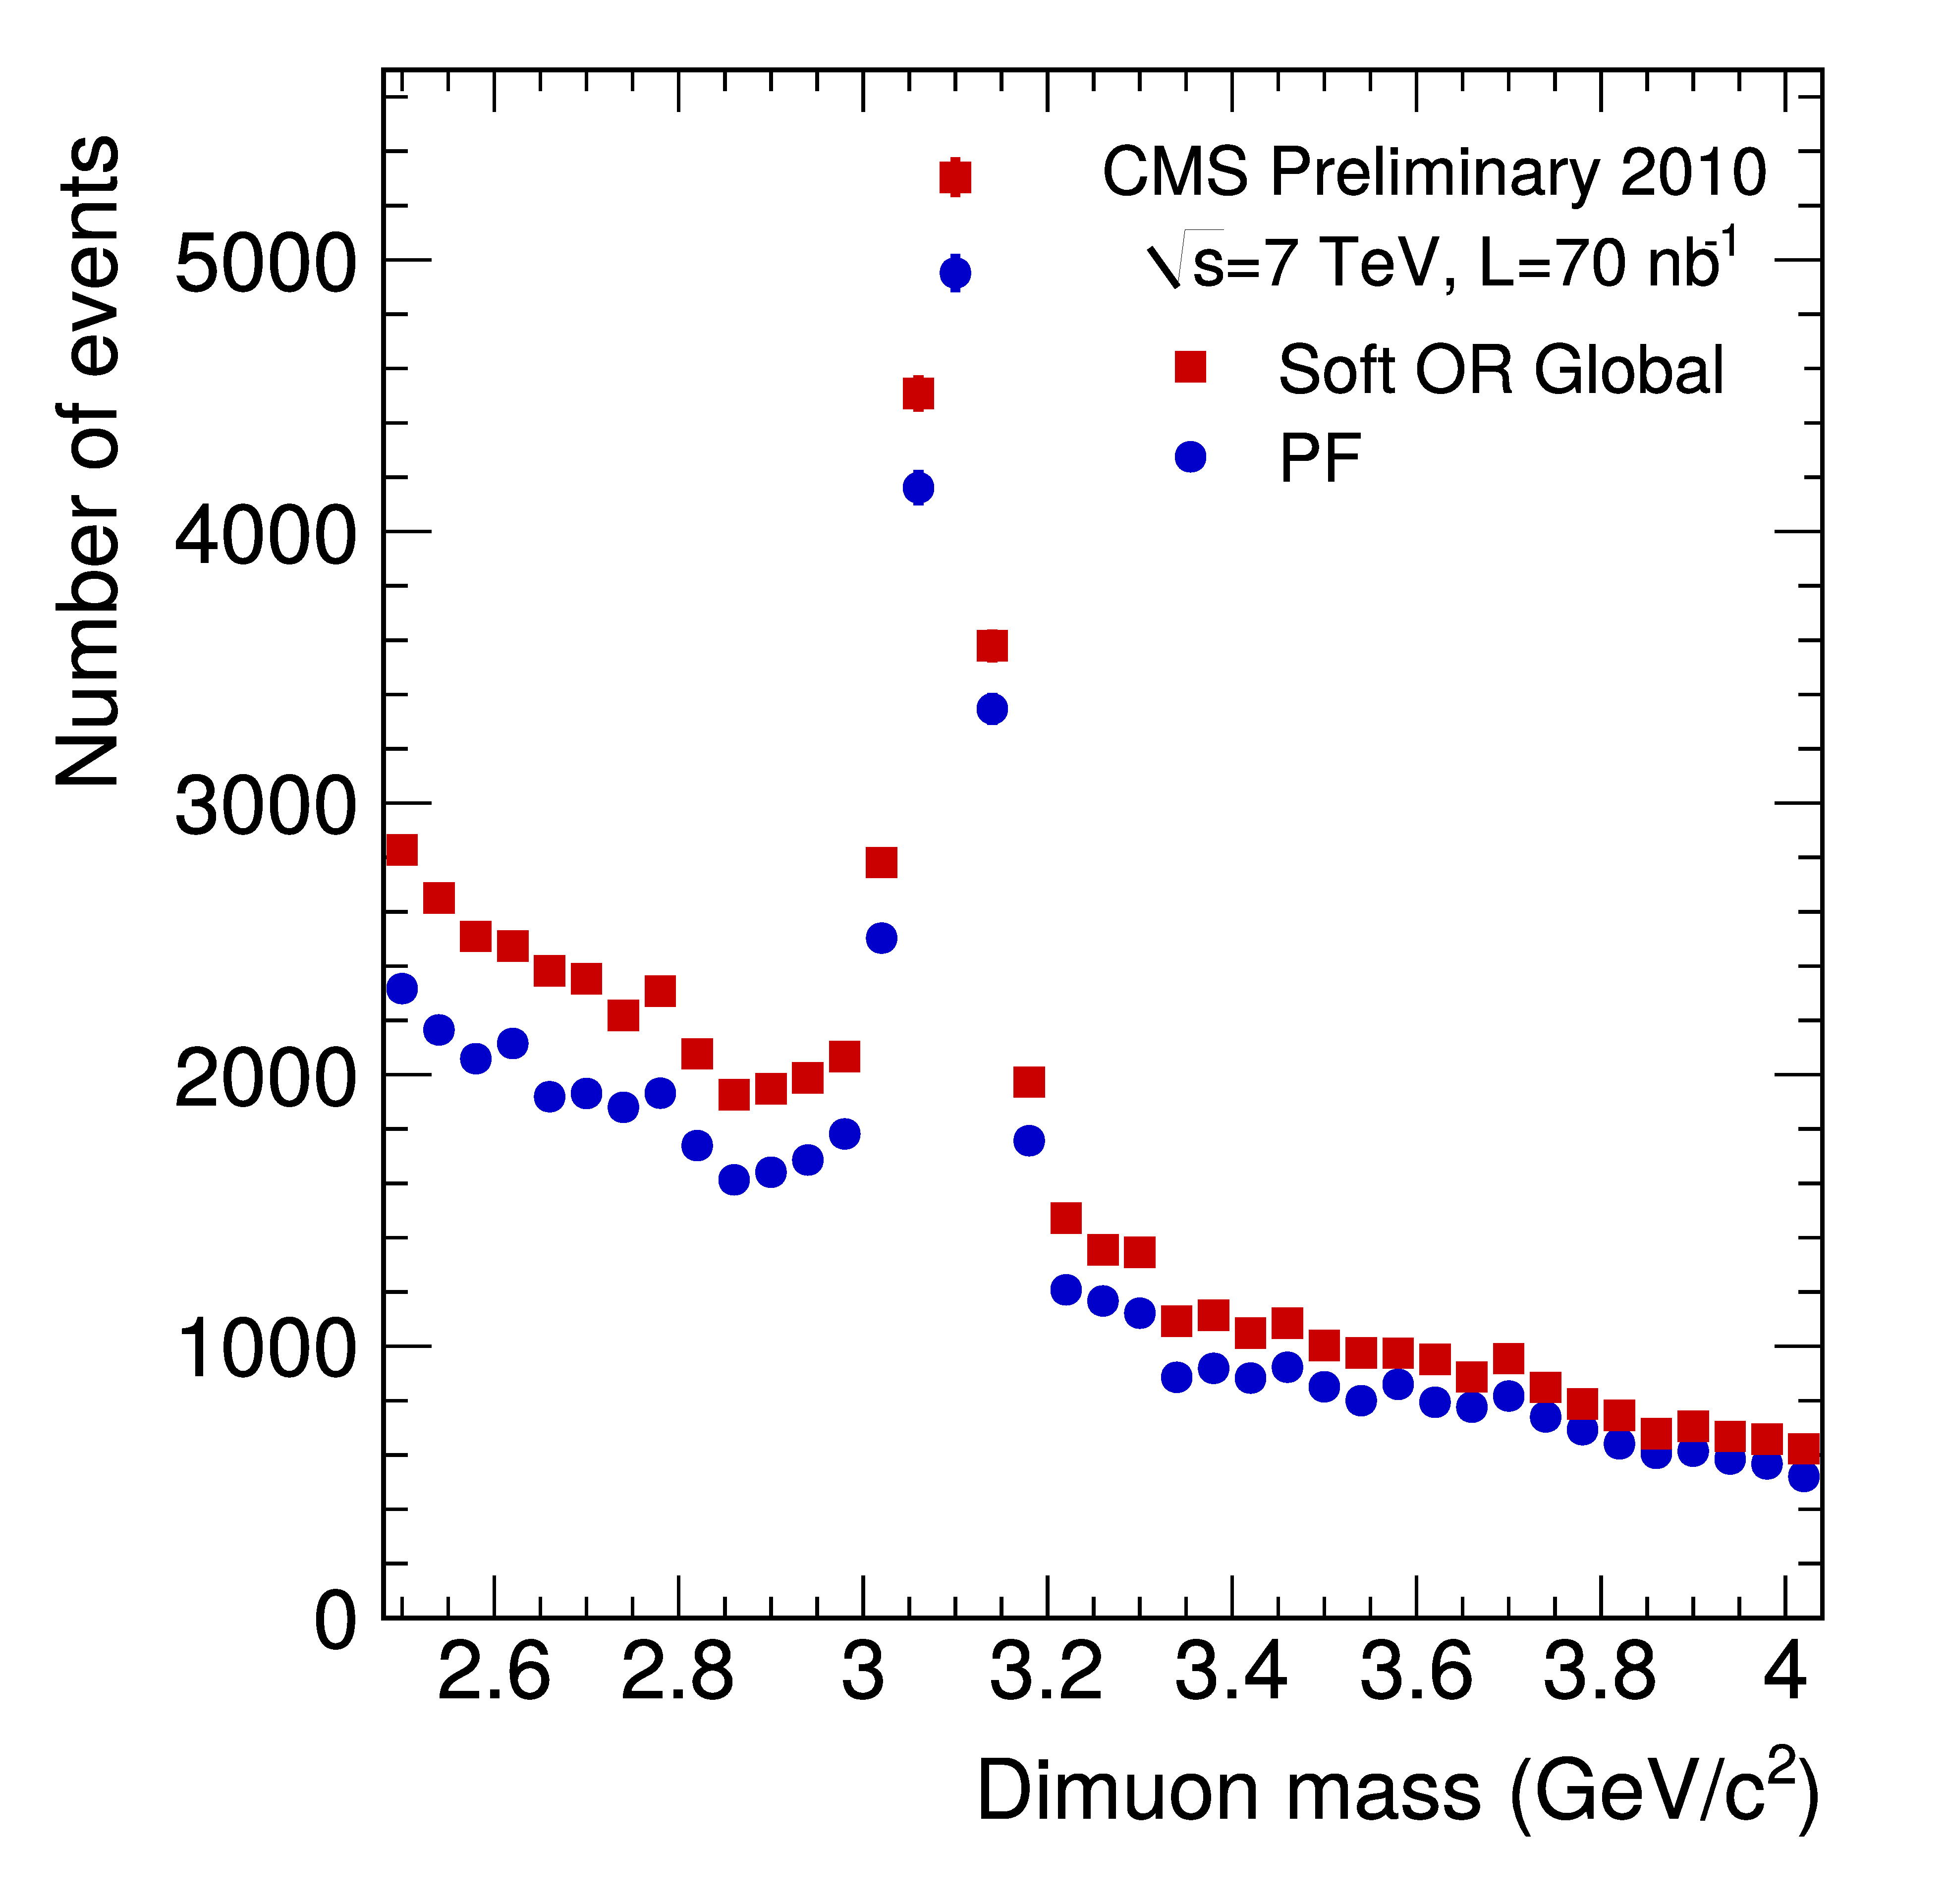
\includegraphics[width=0.4\textwidth]{chapitre3/figs/muons_jspi_mass.pdf}
    \caption{Spectre de masse invariante di-muons reconstruit à l'aide des données 2010, à l'aide de la reconstruction standard des muons (rouge) et à l'aide de la reconstruction \emph{particle-flow} (bleu).}
    \label{fig:muons_jspi}
\end{figure}

Pour chaque muon reconstruit, on enlève les blocs \emph{particle-flow} correspondant de la liste des blocs disponibles, et on procède ensuite à la reconstruction des électrons.

\subsubsection{Reconstruction des électrons}

L'algorithme de reconstruction des traces de CMS (voir \cref{sec:tracks_reconstruction}) est optimisé pour reconstruire les traces des muons. Les électrons étant beaucoup plus léger que les muons, la radiation Bremsstrahlung est amplifié par un facteur $\left( \sfrac{m_\mu}{m_e} \right)^4 \simeq \num{1.83e9}$, ce qui met en défaut l'algorithme de reconstruction des traces. En effet, la trajectoire des électrons peut changer brusquement lors de l'émission d'un photon Bremsstrahlung, et l'algorithme de reconstruction n'arrive plus à suivre la trajectoire abrupt de l'électron. En cas d'émission d'un photon de basse énergie, l'algorithme peut arriver à reconstruire quand même la trajectoire de l'électron, mais au prix d'une grande incertitude et d'un $\chi^2$ grand.

Un algorithme dédié a été développé par CMS pour contrer ces problèmes \citep{pf,cms_pf_leptons,cms_pf_electrons}. La trajectoire de l'électron est redéfinie, en modélisant le rayonnement Bremsstrahlung par une somme de gaussienne (algorithme GSF, pour \emph{Gaussian Sum Filter}. Le nombre de paramètres libres étant important (plus d'une dizaine), l'algorithme est capable de suivre les brusques changement de trajectoire, et ainsi procure une bien meilleure estimation de l'impulsion des électrons. En contre-partie, cet algorithme est très gourmand en ressource (environ \SI{200}{\ms} par trace), et ne peut donc être utilisé que sur un nombre réduit de traces. Il est alors nécessaire d'effectuer une pré-sélection dans les traces existantes afin d'extraire celles qui ont le plus de chance d'être causée par un électron.

La pré-sélection des électrons exploite les caractéristiques des traces. Lorsque la radiation Bremsstrahlung est négligeable, l'algorithme classique reconstruit une trace et on trouve un bloc \emph{particle-flow} associé. Si le rapport $E/p$ est proche de l'unité, la trace est sélectionnée. Quand le rayonnement Bremsstrahlung n'est pas négligeable, deux cas sont possibles :
\begin{itemize}
    \item L'algorithme de reconnaissance de traces échoue lors d'un changement abrupt de trajectoire. La trace résultante contient alors un petit nombre de \emph{hits}.
    \item L'algorithme de reconnaissance de traces reconstruit une trace, mais le $\chi^2$ associé est grand.
\end{itemize}

\begin{figure}[tbp]
    \centering
    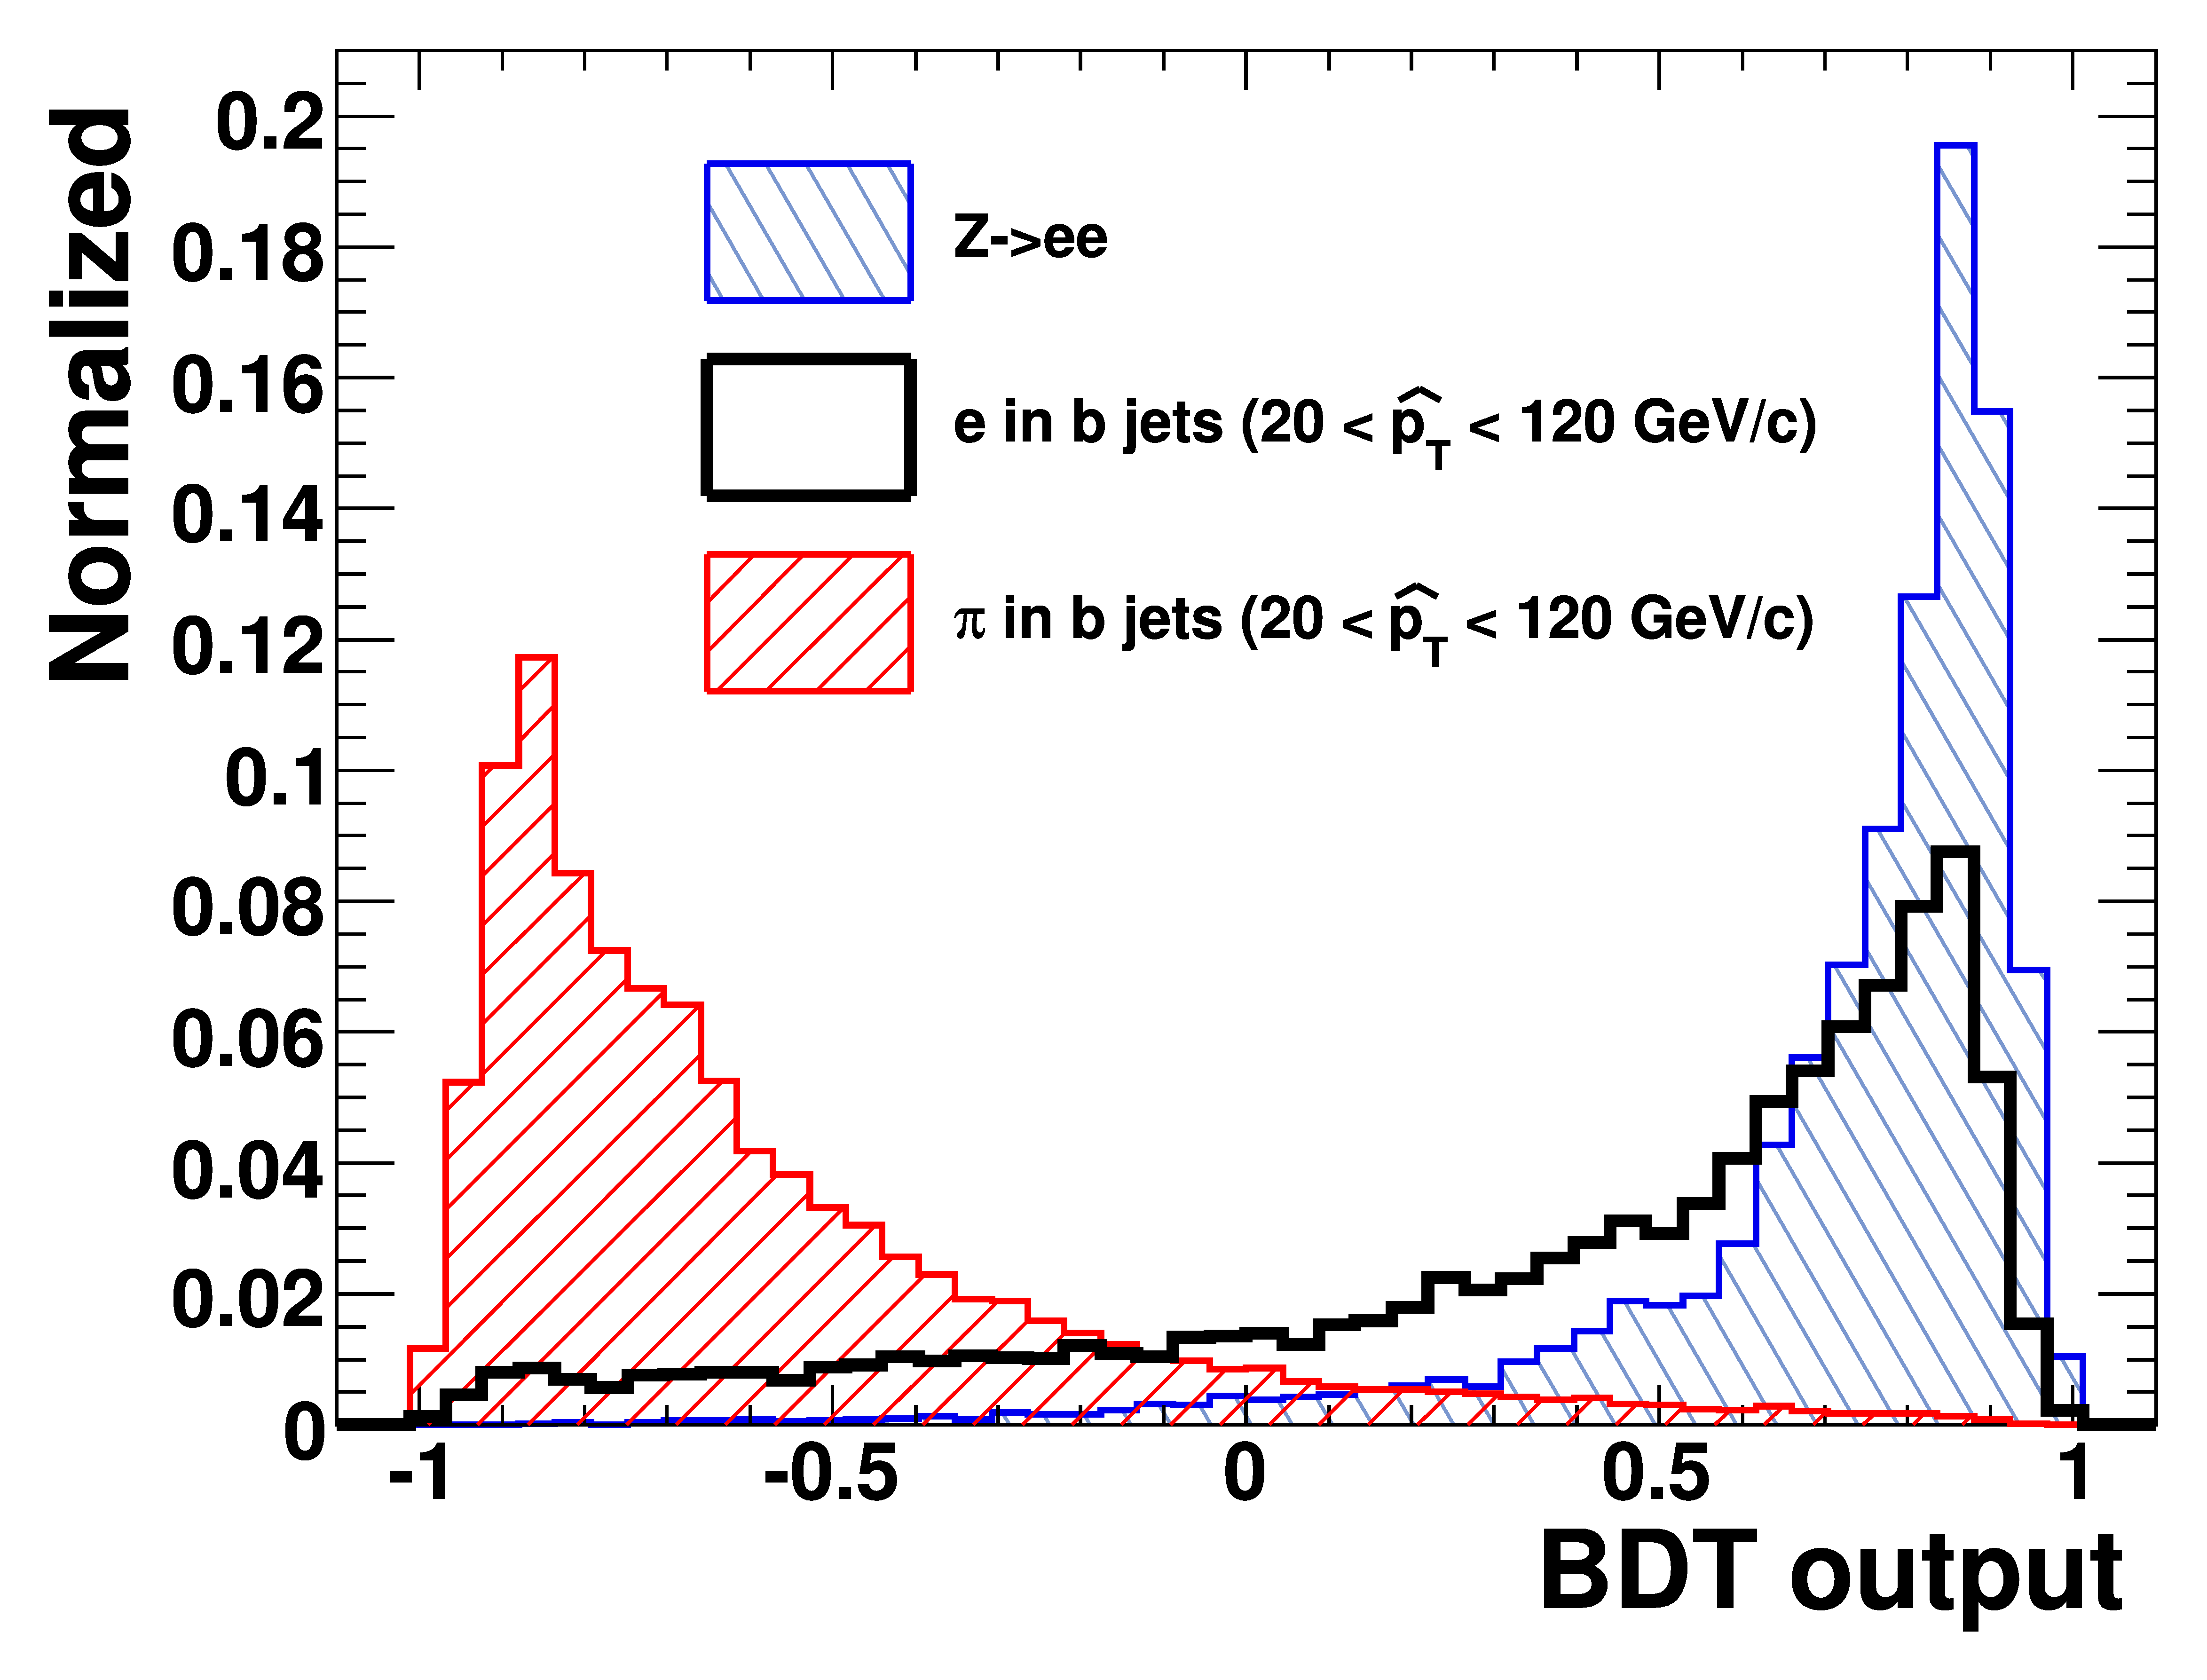
\includegraphics[width=0.5\textwidth]{chapitre3/figs/bdt_electron.pdf}
    \caption{Sortie de l'algorithme de pré-sélection des électrons, pour des électrons isolés (bleu), des électrons dans des jets de $b$ (noir) et pour des pions dans des jets de $b$.}
    \label{fig:bdt_electron}
\end{figure}

Une sélection est appliquée en utilisant ces deux variables, puis une interpolation GSF (avec seulement 5 paramètres libres, donc moins contraignante) est effectuée si la trace passe la sélection. Le $\chi^2$ de cette interpolation ($\chi^2_{GSF}$), le rapport $\chi^2_{KF} / \chi^2_{GSF}$, le nombre de \emph{hits} ainsi que le facteur de qualité du lien ECAL -- trace sont utilisés en entrée d'un algorithme d'arbres de décisions boostés. La sortie de cet algorithme est présentée \cref{fig:bdt_electron}. On peut voir l'excellente discrimination entre les électrons isolés et les pions, et la bonne séparation entre les électrons non isolés et les pions. On considère le candidat comme un électron si la sortie de l'algorithme est supérieur à \num{-0.1} \citep{cms_pf_electrons}. Dans ce cas, les blocs \emph{particle-flow} sont retirés de la liste des blocs disponibles.